This section introduces our implementation of D-Cube algorithm of finding dense block. To be specific, this section describes how to manage data with SQL and how to implement D-Cube algorithms with Python and SQL code.
\subsection{Notations and Symbols}
This following table introduces symbols frequently used in the paper.
 
\begin{table}[h!]
\centering
\begin{tabular}{|p{3cm}|p{10cm}|}
 \hline
 Symbol & Description \\ [0.5ex] 
 \hline\hline
 R & Relation table: an N-way tensor table includes N columns.  Each column represents a dimension attribute. \\
 \hline
 Rn & Table with 1 column which contains distinct values of the n-th attribute of R \\ 
 \hline
 MassR & mass of R (or B) \\ 
 \hline
 $MassB_{a,n}$ & attribute value mass of a in dimension n \\[1ex]
 \hline
\end{tabular}
\caption{Table of Notations and Symbols}
\label{table:1}
\end{table}

\subsection{Generic SQL Codes}
This section describes general SQL method for general data management and manipulation of tables which are used across different algorithms.

\begin{itemize}
    \item \textbf{TableDropCreate} \\
    If table $T$ exists, drop it.
    \begin{algorithmic}
    \STATE DROP TABLE $T$
    \end{algorithmic} 
    Create a new table $T$ with column format $F$.
    \begin{algorithmic}
    \STATE CREATE TABLE $T$ ($F$)
    \end{algorithmic} 
    \item \textbf{LoadTableFromFile} \\
    Load data in file $file$ to table $T$ with column format $F$. 
    \begin{algorithmic}
    \STATE COPY $T$ ($F$) FROM $file$ DELIMITER AS $delim$ CSV
    \end{algorithmic}
    \item \textbf{CopyTable} \\ 
    Create Table $T2$ and insert all data from $T1$.
    \begin{algorithmic}
    \STATE CREATE TABLE $T2$ AS TABLE $T1$
    \end{algorithmic}
    \item \textbf{DistinctAttributeValue} \\
    Computes the set of distinct values on attribute $A$ of table $T$ and save them into table $Tn$.
    \begin{algorithmic}
    \STATE TableDropCreate($Tn$)
    \STATE INSERT INTO $Tn$($A$) SELECT DISTINCT ON ($A$) $A$ FROM $T$
    \end{algorithmic}
    \item \textbf{Mass} \\
    Compute the mass of table $T$. We assume all the tuples in $T$ has a measure attribute equals to 1.
    \begin{algorithmic}
    \STATE SELECT count(*) FROM $T$
    \end{algorithmic}
    \item \textbf{DeleteRows} \\
    Delete rows in Table $T$ with $condition$.
    \begin{algorithmic}
    \STATE DELETE FROM $T$ WHERE $condition$
    \end{algorithmic}
    \item \textbf{InsertRow} \\
    Insert a $newEntry$ into Table $T$.
    \begin{algorithmic}
    \STATE INSERT INTO $T$ VALUES ($newEntry$)
    \end{algorithmic}
\end{itemize}

\subsection{D-Cube Algorithms}
This section describes the implementation of D-Cube algorithms in Python and SQL. D-Cube algorithms are efficient and accurate to find dense blocks. This method is widely used in different practical tasks, such as finding malicious attacks in the network transmission and finding abnormal following relationship in social network data.

\subsubsection{Overall Structure of D-Cube (Algorithm 1)}
This algorithm describes the over structure of D-CUBE. It takes command line input as arguments. The table \ref{table:2} shows description of these arguments.
 
\begin{table}[h!]
\centering
\begin{tabular}{|p{2cm}|p{2cm}|p{4cm}|p{5cm}|}
 \hline
 notation & type & requirement & description \\ [0.5ex] 
 \hline\hline
 --file & string & Required & Full path to the data file to load from. \\ 
 --delim & string & default=',' & Delimiter that separate the columns in the input file. \\
 --N & integer & Required & Number of dimension attributes.\\
 --k & integer & Required & Number of dense blocks we aim to find. \\
 --density & string & default='arithmetic' & Density measures. Support arithmetic, geometric and suspiciousness. \\
 --selection & string & default='density' & Dimension selection policy. Support density and cardinality.\\ [1ex] 
 \hline
\end{tabular}
\caption{Table of arguments}
\label{table:2}
\end{table}

The main idea of this algorithm is to find each dense block one by one. It keeps a static copy of the original relation table. After each block $B$ is found, tuples are removed from relation table to avoid duplication. However, when construct the final dense block, it select tuples from the original relation table such that we can get overlaped dense blocks.

\begin{algorithm}[H]
\SetKwInOut{Input}{Input}
\SetKwInOut{Output}{Output}
\SetAlgoLined
\Input{Arguments}
\Output{k dense block tables and a report table}
\begin{algorithmic}
 \STATE $TableDropCreate(R)$
 \STATE $TableDropCreate(ReportTable)$
 \STATE $LoadTableFromFile(R)$
 \STATE $CopyTable(ORI, R)$ 
 \STATE \For{n in range(N)} {
    \STATE $DistinctAttributeValue(Rn)$
 }
 \STATE $TableDropCreate(ResultTable)$ 
 \STATE \For{i in range(k)}{
    \STATE $MassR \gets Mass(R)$
    \STATE $Bn \gets find\_single\_block(R,Rn,MassR,density)$  
    \COMMENT{$\#See\ Algorithm\ 2$}
    \STATE $DeleteFromBlock(R, Bn)$
    \STATE $BlockCreateInsert(ResultTable\_i, ORI, Bn)$
    \STATE $Update(ReportTable)$
 }
\end{algorithmic}
 \caption{D-CUBE}
\end{algorithm} 

Details of special functions in Algorithm 1 are listed below:
\begin{itemize}
    \item \textbf{DeleteFromBlock} \\
    Delete block $B$ from relation $R$. Delete tuples of $R$ that all attributes are in $Bn$.
    \begin{algorithmic}
    \STATE DELETE FROM $R$ USING $B0$, ... ,$Bn$ \\
    WHERE $R$.$A0$=$B0$.$A0$ AND ... AND $R$.$An$=$Bn$.$An$
    \end{algorithmic}
    \item \textbf{BlockCreateInsert} \\
    Create the table of block in $ORI$ formed by the same attribute values forming $Bn$.
    \begin{algorithmic}
    \STATE INSERT INTO $ResultTable\_i$($A$) \\
    SELECT $ORI$.$A0$, ..., $ORI$.$An$ FROM $ORI$, $B0$, ..., $Bn$\\
    WHERE $ORI$.$A0$=$B0$.$A0$ AND ... AND $ORI$.$An$=$Bn$.$An$ \\
    ORDER BY $A0$,...,$An$
    \end{algorithmic}
\end{itemize}

\subsubsection{Single Block Detection (Algorithm 2)}
This algorithm describes how to find each dense block from the given relation. The main idea is to order the attribute values based on block density. We can iterate to select dimension and delete attribute values. Because of the order of attribute values, we can get the optimal number of attribute to remove where we could get maximum block density. 

\begin{algorithm}[H]
\SetKwInOut{Input}{Input}
\SetKwInOut{Output}{Output}
\SetAlgoLined
\Input{$R$, $Rn$, $MassR$, $density$}
\Output{tables of attribute values forming a dense block}
\begin{algorithmic}
 \STATE $CopyTable(B, R)$
 \STATE $MassB \gets MassR$
 \STATE $CopyTable(Bn, Rn)$
 \STATE $BestDensity \gets DensityMeasure(MassB, Bn, MassR, Rn)$   
 \COMMENT{$\#See\ Algorithm\ 3$}
 \STATE $r, Best\_r \gets 1$
 \STATE $TableDropCreate(OrderTable)$
 \STATE \While{$BlockNotEmpty(B)$}{
    \STATE \For{n in range(N)}{
    \STATE $DistinctAttributeValue(Bn)$
    } 
    \STATE $TableDropCreate(AttValMassTable)$
    \STATE $AttValMass(AttValMassTable)$
    \STATE $i \gets SelectDimension()$ 
    \COMMENT{$\#See\ Algorithm\ 4$}
    \STATE $threshold \gets MassB / MassB_i$
    \STATE $SelectValuesToRemove(D_i)$
    \STATE $CopyTable(D_static, D_i)$
    \STATE \While{$TableNotEmpty(D_i)$}{
        \STATE $a,MassB_{a,i} \gets FetchFirstRow(D_i)$
        \STATE $DeleteRows(D_i)$
        \COMMENT{$\# Delete\ all\ rows\ with\ same\ a\ and\ MassB_{a,i}$}
        \STATE $DeleteRows(B_i)$ 
        \COMMENT{$\# Delete\ a\ from\ B_i$}
        \STATE $MassB \gets MassB - MassB_{a,i}$
        \STATE $density' \gets DensityMeasure(MassB, Bn, MassR, Rn)$ 
        \STATE $InsertRow(OrderTable)$
        \COMMENT{$\# Insert\ a,i,r\ into\ OrderTable$}
        \STATE $r \gets {r + 1}$
        \STATE \If{${{density'}>{BestDensity}}$}{
            \STATE $BestDensity \gets density'$ 
            \STATE $Best\_r \gets r$ 
        }
    }
    \STATE $UpdateBlock(B, D_i)$
 } 
 \STATE $ReconstructBlock(Best\_Bn)$ 
\end{algorithmic}
 \caption{find\_single\_block in D-CUBE}
\end{algorithm}

Details of special functions in Algorithm 2 are listed below:

\begin{itemize}
    \item \textbf{AttValMass}    \\
    Compute attribute value mass $M_{B(a,n)}$. For each dimension $dim$, we calculate number of the tuples in $B$ whose attribute value equals to $a$.
    \begin{algorithmic}
    \STATE INSERT INTO $AttValMassTavle$ \\
        SELECT $dim$, $B$.$A_{dim}$, COUNT(*) AS $AttValMass$ \\ 
        FROM $B_{dim}$ AS A, $B$ WHERE A.$A_{dim}$ = $B$.$A_{dim}$ \\
        GROUP BY $B$.$A_{dim}$"
    \end{algorithmic}
    \item \textbf{SelectValuesToRemove} \\
    Select attribute values to be removed according to table $AttValMassTable$ and $threshold$. Sort the table in an increasing order of attribute mass.
    \begin{algorithmic}
    \STATE  INSERT INTO $D_i$ SELECT $a\_value$, $attrVal\_mass$ \\
    FROM $AttValMassTable$  \\
    WHERE $dimension\_index = i$ AND $attrVal\_mass \leq threshold$ \\
    ORDER BY $attrVal\_mass$
    \end{algorithmic}
    \item \textbf{FetchFirstRow} \\
    Fetch the first row of the $D_i$ table.
    \begin{algorithmic}
    \STATE SELECT $a\_value$, $attrVal\_mass$::text \\
    FROM $D_i$ LIMIT 1
    \end{algorithmic}
    \item \textbf{UpdateBlock} \\
    Remove tuples in $B$ whose attribute value $A_i$ is in $D_i$.
    \begin{algorithmic}
    \STATE DELETE FROM $B$ USING $D_i$ \\
    WHERE $B$.$A_i$ = $D_i$.$a\_value$
    \end{algorithmic}
    \item \textbf{ReconstructBlock} \\
    Reconstruct block $Best\_B$ with attribute values that maximize block density. These attribute values should have order greater than $Best\_r$.
    \begin{algorithmic}
    \STATE INSERT INTO $Best\_Bn$ \\
        SELECT A.$An$ FROM $R$ AS A, $OrderTable$ AS B\\ 
        WHERE A.$An$ = B.$a\_value$ AND \\
        B.${{order\_a\_i} \geq {Best\_r}}$ \\
        AND B.$dimension\_index$ = $n$
    \end{algorithmic}
\end{itemize}

\subsubsection{Density Measures (Algorithm 3)}
This algorithm support three methods to calculate block density: Arithmetic Average Mass, Geometric Average Mass and Suspiciousness.

\begin{algorithm}[H]
\caption{DensityMeasure}
    \SetKwInOut{Input}{Input}
    \SetKwInOut{Output}{Output}
    \SetAlgoLined
    \Input{$MassB$, $Bn$, $MassR$, $Rn$, $method$}
    \Output{density of the dense block}
    \begin{algorithmic}  
    \STATE \If{$method=Arithmetic$}{                                
        \STATE $sum \gets 0$
        \STATE \For{n in range(N)}{
            \STATE $sum = {{sum} + {Mass(Bn)}}$
        } 
        \STATE $density = MassB / sum * N$
    }
    \If{$method = Geometric$}{
        \STATE $product \gets 1$
        \STATE \For{n in range(N)}{
            \STATE $product = {{product} * {Mass(Bn)}}$
         } 
         \STATE $power = pow(product, \frac{1}{N})$
         \STATE $density = MassB / power$
     }
    \STATE \If{$method=Suspiciousness$}{
        \STATE $ratio \gets {MassB}/{MassR}$ 
        \STATE $density = MassB * (log(ratio)-1)$
        \STATE $ratioProduct \gets 1$ 
        \STATE \For{n in range(N)}{
            \STATE $ratioProduct = {{ratioProduct} * {Mass(Bn)} / {Mass(Rn)}}$
        } 
        \STATE $density = density + MassR * ratioProduct - MassB * log(ratioProduct)$
    }
    \end{algorithmic}
\end{algorithm}

\subsubsection{Dimension Selection (Algorithm 4)}
This algorithm support two policy to select dimension for attribute value removal in Algorithm 2. They are select\_dimension by cardinality and select\_dimension by density.

\begin{algorithm}[H]
\SetKwInOut{Input}{Input}
\SetKwInOut{Output}{Output}
\SetAlgoLined
\Input{$Bn$, $N$, $policy$}
\Output{a dimension in [$N$]}
\begin{algorithmic}
 \STATE \If{$policy = cardinality$}{
    \STATE $dim \gets -1$
    \STATE $maxMass \gets -1$
    \STATE \For{n in range(N)}{
        \STATE $currMass = Mass(Bn)$
        \STATE \If{${{currMass} > {maxMass}}$}{
        \STATE $maxMass=currMass$
        \STATE $dim = n$
        }
     } 
 }
\STATE \If{$policy = density$}{
    \STATE $BestDensity \gets -\infty$
    \STATE $dim \gets 1$
    \STATE \For{$i\ in\ range(N)$}{
        \STATE \If{$BlockNotEmpty(B_i)$}{
            \STATE $threshold \gets MassB / MassB_i$ 
            \STATE $SelectValuesToRemove(D_i)$
            \STATE $delta \gets DcubeSum(D_i)$
            \STATE $MassB' \gets MassB-delta$
            \STATE $B_i' \gets UpdateBlock(B_i, D_i)$
            \STATE $Switch\ B_i'\ and\ B_i$
            \STATE $density' \gets DensityMeasure(MassB, Bn, MassR, Rn)$
            \STATE $Switch\ B_i'\ and\ B_i$
            \STATE \If{${{density'}>{BestDensity}}$}{
                \STATE $BestDensity \gets density'$
                \STATE $dim \gets i$
                }
        }
    }
 }
\end{algorithmic}
\caption{select\_dimension}
\end{algorithm}

Details of special functions in Algorithm 2 are listed below:
\begin{itemize}
    \item \textbf{DcubeSum} \\
    Calculate sum of attribute value masses in $D$
    \begin{algorithmic}
    \STATE SELECT SUM($attrval\_mass$) FROM $D$
    \end{algorithmic}
\end{itemize}

\subsubsection{Bucketize Time}
Time attribute is very special in finding dense block problem. For the purpose of grouping data into meaningful time slots, we use bucketize time method to construct time buckets by hour.
The main idea is to update relation table after loaded from csv file by ignoring minutes with regular expression. 
\begin{algorithmic}
\STATE UPDATE $R$ SET $time\_stamp$ = SUBSTRING($time\_stamp$ from '.*:')
\end{algorithmic}

\subsubsection{Unit Tests}
We construct a test dataset of 798 rows by manuly select dense blocks labeled as 'smurf' in 'darpa\_with\_label' and the rest of the tensor have tiny diversity. The table \ref{table:test} shows description of these arguments.
 
\begin{table}[h!]
\centering
\begin{tabular}{|p{5cm}|p{10cm}|}
 \hline
 Function Name & Expected Result \\ [0.5ex] 
 \hline\hline
 TableDropCreate & Drop old table with same name and create a new empty table. \\ 
 LoadTableFromFile & Load relation table from csv file. Get a table of $798$ rows. \\
 CopyTable & A new table same as the source table.\\
 DistinctAttributeValue & Distinct attribute values of the relation table. Get three tables with $420$, $79$ and $21$ rows. \\
 Mass & Get total row number of the table. Should return 798 for relation table. \\
 DeleteRows & All tuples under condition are removed \\
 InsertRow & A new row is appended in the table \\
 DeleteFromBlock & All tuples with specific attributes are deleted. \\
 BlockCreateInsert & Get result dense block table. \\
 AttValMass & Get a table of attribute value, dimension and attribute value mass. \\
 SelectValuesToRemove & Get a table of attribute value and attribute value mass. No attribute value mass is greater than threshold. \\
 FetchFirstRow & Get attribute value $a$ and corresponding attribute value mass \\ 
 UpdateBlock & A new block table whose tuples don't have same attribute values in table $D$. \\
 ReconstructBlock & Get a dense block table.\\
 DensityMeasure & Three density values that consistent with the manual calculation results. \\
 DimensionSelection & Get a dimension for removal. According to our testset, the first selection should return dimension $0$.\\ [1ex] 
 \hline
\end{tabular}
\caption{Table of unit tests}
\label{table:test}
\end{table}

\subsection{Optimization (T3)}
In this section, we implement two different methods to update tables. One is to copy relation table for block detection and actually delete dense block tuples in the relation table. The other one is to add a marker column to mark removed tuples. This method needs to update the markers instead of deleting records in the table. We also explore the influence of various indexing options. We do several experiments to compare the total running time under different methods.
\subsubsection{'Copy' Method}
In the 'Copy' Method, we firstly load the relation table from the csv file. For each iteration of finding a single dense block, we need to copy the whole relation table to block table. After we get the sets of attribute values forming a dense block, we need to actually delete the records with same attribute values in the relation table. \\
The advantages of this method include: 
\begin{itemize}
    \item Since all data are up to date, we don't need to judge if the records were deleted when we want to select some records from the table.
    \item We can save space because we actually delete all unnecessary data.
\end{itemize}
The downsides of this method include:
\begin{itemize}
    \item Deletion is often very slow because the database needs to change the size of the table and actually remove the data.
    \item We can't get the data back after deletion
\end{itemize}
 
\subsubsection{'Mark' Method}
In the 'Mark' Method, we add an empty column called 'Marker' after we load the relation table from the csv file. For each iteration of finding a single dense block, we need to select all the records in the relation table with NULL in Marker. Operations of getting distinct attribute values and calculating block mass will also need to check the value of Marker. After we get the sets of attribute values forming a dense block, we need to update the Markers of related records to 0. \\
The advantages of this method include:
\begin{itemize}
    \item Using a flag to mark the deletion option will be faster than actually delete the records in the table.
    \item We can get the data back after deletion.
\end{itemize}
The downsides of this method include:
\begin{itemize}
    \item We need to check the markers when we try to copy the relation table, compute distinct attribute values of relation table and calculating mass. This makes codes more complicated and takes more time because database needs to check more constraints.
    \item Waste more space because the deleted records are still in the table.
\end{itemize}

\subsubsection{Indexing}
We monitor the running time of each module and we figure out that most of time goes to three parts: 
\begin{itemize}
    \item In the algorithm 2: Single Block Detection, it takes some time to form the set to be removed $D_i$.
    \item In the algorithm 2: Single Block Detection, it takes some time to reconstruct sets of attribute values after we have the order table.
    \item In the algorithm 1: Overall Structure of D-Cube, it takes some time to reconstruct the final dense block.
\end{itemize}
Thus, we decide to create index on $AttValMassTable$, $OrderTable$ and $ORI$. We used 3 different methods of creating index: btree, gist, and gin. We also do experiments to explore which option performs best. \\

\subsubsection{Experimental Comparison}
\begin{figure}[h]
    \begin{center}
      \makebox[\textwidth]{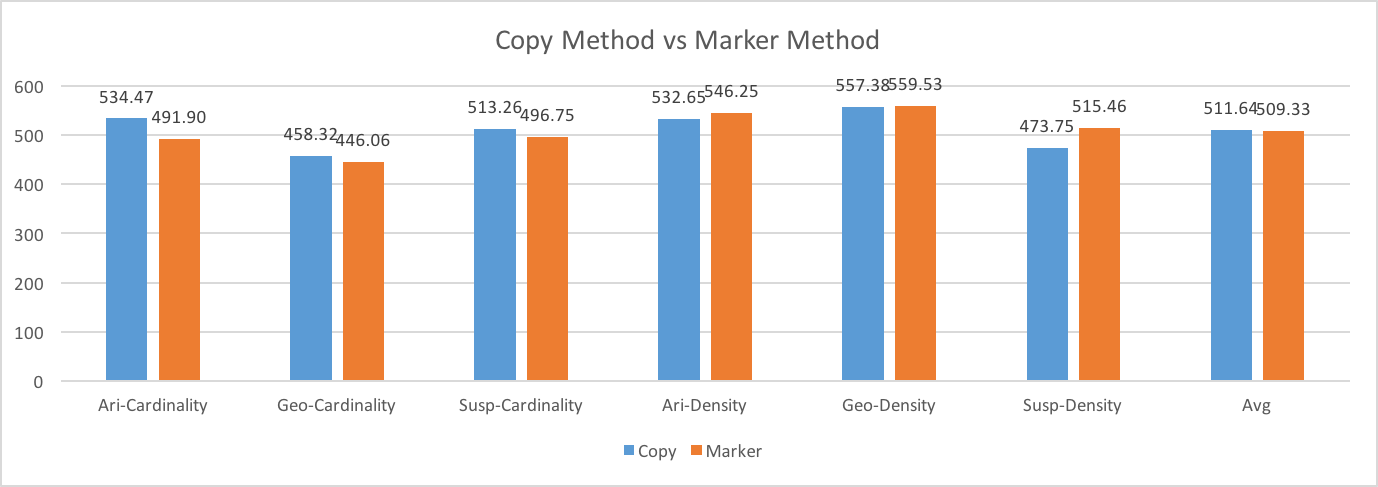
\includegraphics[width=\textwidth]{CopyMarker.png}}
    \end{center}
    \caption{Copy Method vs Marker Method}
    \label{fig:CopyMarker}
\end{figure}
We compare the total running times of Copy Method and Marker Method under different parameter settings. The result in Figure \ref{fig:CopyMarker} shows that Marker Method could reduce the running time on average. However, in some cases, for example, when we use suspiciousness as diversity measurement and density as selection policy, the Copy Method beats Marker Method. This is because Marker Method wastes too much time on checking flags for select operation. The time spent on checking marks exceeds the time saved for deletion.
\begin{figure}[h]
    \begin{center}
      \makebox[\textwidth]{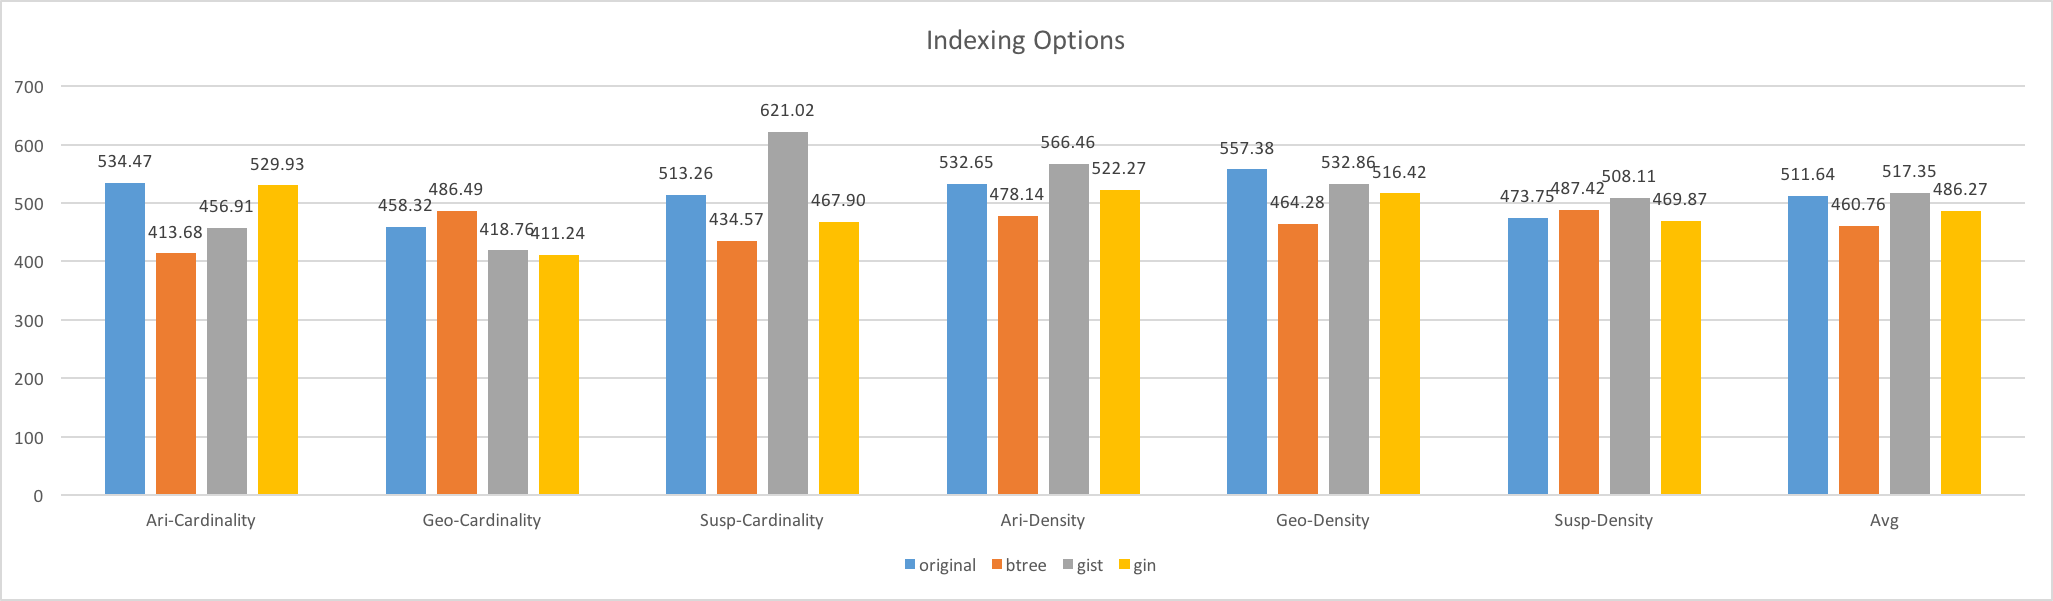
\includegraphics[width=\textwidth]{indexing.png}}
    \end{center}
    \caption{Indexing Options}
    \label{fig:Indexing}
\end{figure} \\

We also compare the total running times of 3 indexing options under different parameter settings. The result in Figure \ref{fig:Indexing} shows that in most cases, indexing will help reduce running time. In the worst case, the time spent on creating index sometimes exceeds the time saved by indexing. We think indexing will help a lot on larger datasets. The experiment result also indicates that the btree option is the best choice since it has lowest average running time.\\